\chapter{Dữ liệu ViMedAQA}
\section{Mô tả bộ dữ liệu}
ViMedAQA \cite{tran2024vimedaqa} là bộ dữ liệu hỏi đáp trừu tượng tiếng Việt trong miền y khoa chất lượng cao. Khác biệt với các bộ dữ liệu hỏi đáp trích xuất (Extractive Question Answering) thông thường khi câu trả lời chỉ là một phân đoạn văn bản (span) được cắt trực tiếp từ ngữ cảnh, ViMedAQA tập trung vào bài toán hỏi đáp trừu tượng (Abstractive Question Answering). Trong miền y khoa, câu trả lời trừu tượng mang lại giá trị thực tiễn rất cao vì bệnh nhân và chuyên gia y tế thường yêu cầu những phản hồi được tổng hợp, diễn giải một cách tự nhiên và mạch lạc từ nhiều nguồn thông tin khác nhau. 

Mỗi mẫu dữ liệu trong ViMedAQA bao gồm bốn trường thông tin cốt lõi:
\begin{itemize}
    \item \textbf{Câu hỏi (Question):} Các truy vấn y tế bằng tiếng Việt tự nhiên do người dùng đặt ra, xoay quanh các triệu chứng, phương pháp điều trị, dược phẩm, hoặc kiến thức y học phổ thông.
    \item \textbf{Ngữ cảnh (Context):} Phân đoạn kiến thức y khoa đáng tin cậy được trích xuất từ các tài liệu chuyên ngành, bài báo y học uy tín hoặc hướng dẫn lâm sàng chính thức. Ngữ cảnh này đóng vai trò là nguồn tri thức nền tảng để trả lời câu hỏi.
    \item \textbf{Câu trả lời (Answer):} Câu trả lời chuẩn mực do các chuyên gia y tế hoặc người biên soạn có chuyên môn xây dựng. Câu trả lời này được tổng hợp và diễn đạt lại từ ngữ cảnh một cách ngắn gọn, súc tích và dễ hiểu đối với người bệnh.
    \item \textbf{Chủ đề (Topic):} Nhãn số phân loại chủ đề y khoa tương ứng (gồm 4 chủ đề từ 0 đến 3), giúp mô hình hóa phân phối của các chuyên khoa khác nhau.
\end{itemize}

\section{Định dạng dữ liệu đầu vào cho Seq2Seq}
Để huấn luyện và đánh giá các mô hình Sequence-to-Sequence (Seq2Seq) như ViT5 \cite{phan2022vit5} và BARTpho \cite{tran2021bartpho}, dữ liệu cần được chuẩn hóa về một định dạng chuỗi thống nhất. Định dạng này giúp mô hình phân biệt rõ ràng giữa câu hỏi cần trả lời và ngữ cảnh tri thức đi kèm. Cụ thể, định dạng đầu vào và đầu ra được thiết lập như sau:
\begin{tcolorbox}[colback=codebg, colframe=myblue, title={Định dạng đầu vào/đầu ra thống nhất cho các mô hình Seq2Seq}]
\small\ttfamily
INPUT : question: \{question\} context: \{context\}\par
OUTPUT: \{answer\}
\end{tcolorbox}


\section{Khảo sát dữ liệu thực tế và phân tích EDA}
Quy trình khám phá dữ liệu (Exploratory Data Analysis - EDA) được thực hiện kỹ lưỡng nhằm đánh giá chất lượng phân phối của bộ dữ liệu trước khi huấn luyện. Chúng tôi tiến hành kiểm tra số lượng mẫu, phân phối chủ đề, thống kê độ dài văn bản và đặc biệt là độ trùng khớp từ vựng (vocabulary overlap) giữa câu trả lời và ngữ cảnh. Kết quả thống kê chi tiết của bộ dữ liệu ViMedAQA được tổng hợp tại Bảng~\ref{tab:dataset_stats}.

\begin{table}[H]
\centering
\caption{Thống kê mô tả chi tiết bộ dữ liệu ViMedAQA thực tế}
\label{tab:dataset_stats}
\resizebox{\textwidth}{!}{%
\begin{tabular}{lr}
\toprule
\textbf{Chỉ số thống kê} & \textbf{Giá trị thực nghiệm} \\
\midrule
Tổng số mẫu dữ liệu sạch & 23.553 \\
Kích thước tập huấn luyện (Train split - 80\%) & 18.842 \\
Kích thước tập kiểm định (Validation split - 10\%) & 2.355 \\
Kích thước tập kiểm thử (Test split - 10\%) & 2.356 \\
Số lượng chủ đề y khoa độc lập & 4 \\
Độ trùng khớp từ vựng trung bình (Extractive Overlap) & 82,25\% \\
Độ dài ngữ cảnh trung bình (ViT5 Tokenizer) & 115,36 tokens (Max: 1517) \\
Độ dài ngữ cảnh trung bình (BARTpho Tokenizer) & 121,96 tokens (Max: 1523) \\
\bottomrule
\end{tabular}%
}
\end{table}

Chỉ số độ trùng khớp từ vựng trung bình đạt \textbf{82,25\%} phản ánh đặc tính \textit{semi-abstractive} (bán trừu tượng) của bộ dữ liệu. Mặc dù câu trả lời giữ lại một lượng lớn thuật ngữ chuyên ngành và thực thể y học quan trọng từ ngữ cảnh để đảm bảo tính chính xác khoa học, cấu trúc câu vẫn được tái cấu trúc và viết lại một cách tự nhiên. Thêm vào đó, sự khác biệt về độ dài token trung bình giữa hai bộ mã hóa (115,36 của ViT5 và 121,96 của BARTpho) xuất phát từ cách tiếp cận phân tách từ ngữ của các tokenizer: ViT5 sử dụng SentencePiece mức âm tiết, trong khi BARTpho sử dụng tokenizer cấp từ (word-level) dựa trên thư viện PyVi làm giàu thông tin ngữ nghĩa nhưng tạo ra các chuỗi dài hơn khi gặp từ chuyên ngành ghép nối bằng dấu gạch dưới (\texttt{\_}).

Để trực quan hóa sự phân phối độ dài của các trường dữ liệu quan trọng, chúng tôi vẽ biểu đồ phân phối độ dài của câu hỏi, ngữ cảnh và câu trả lời trong tập dữ liệu (xem Hình~\ref{fig:length_dist}).

\begin{figure}[H]
    \centering
    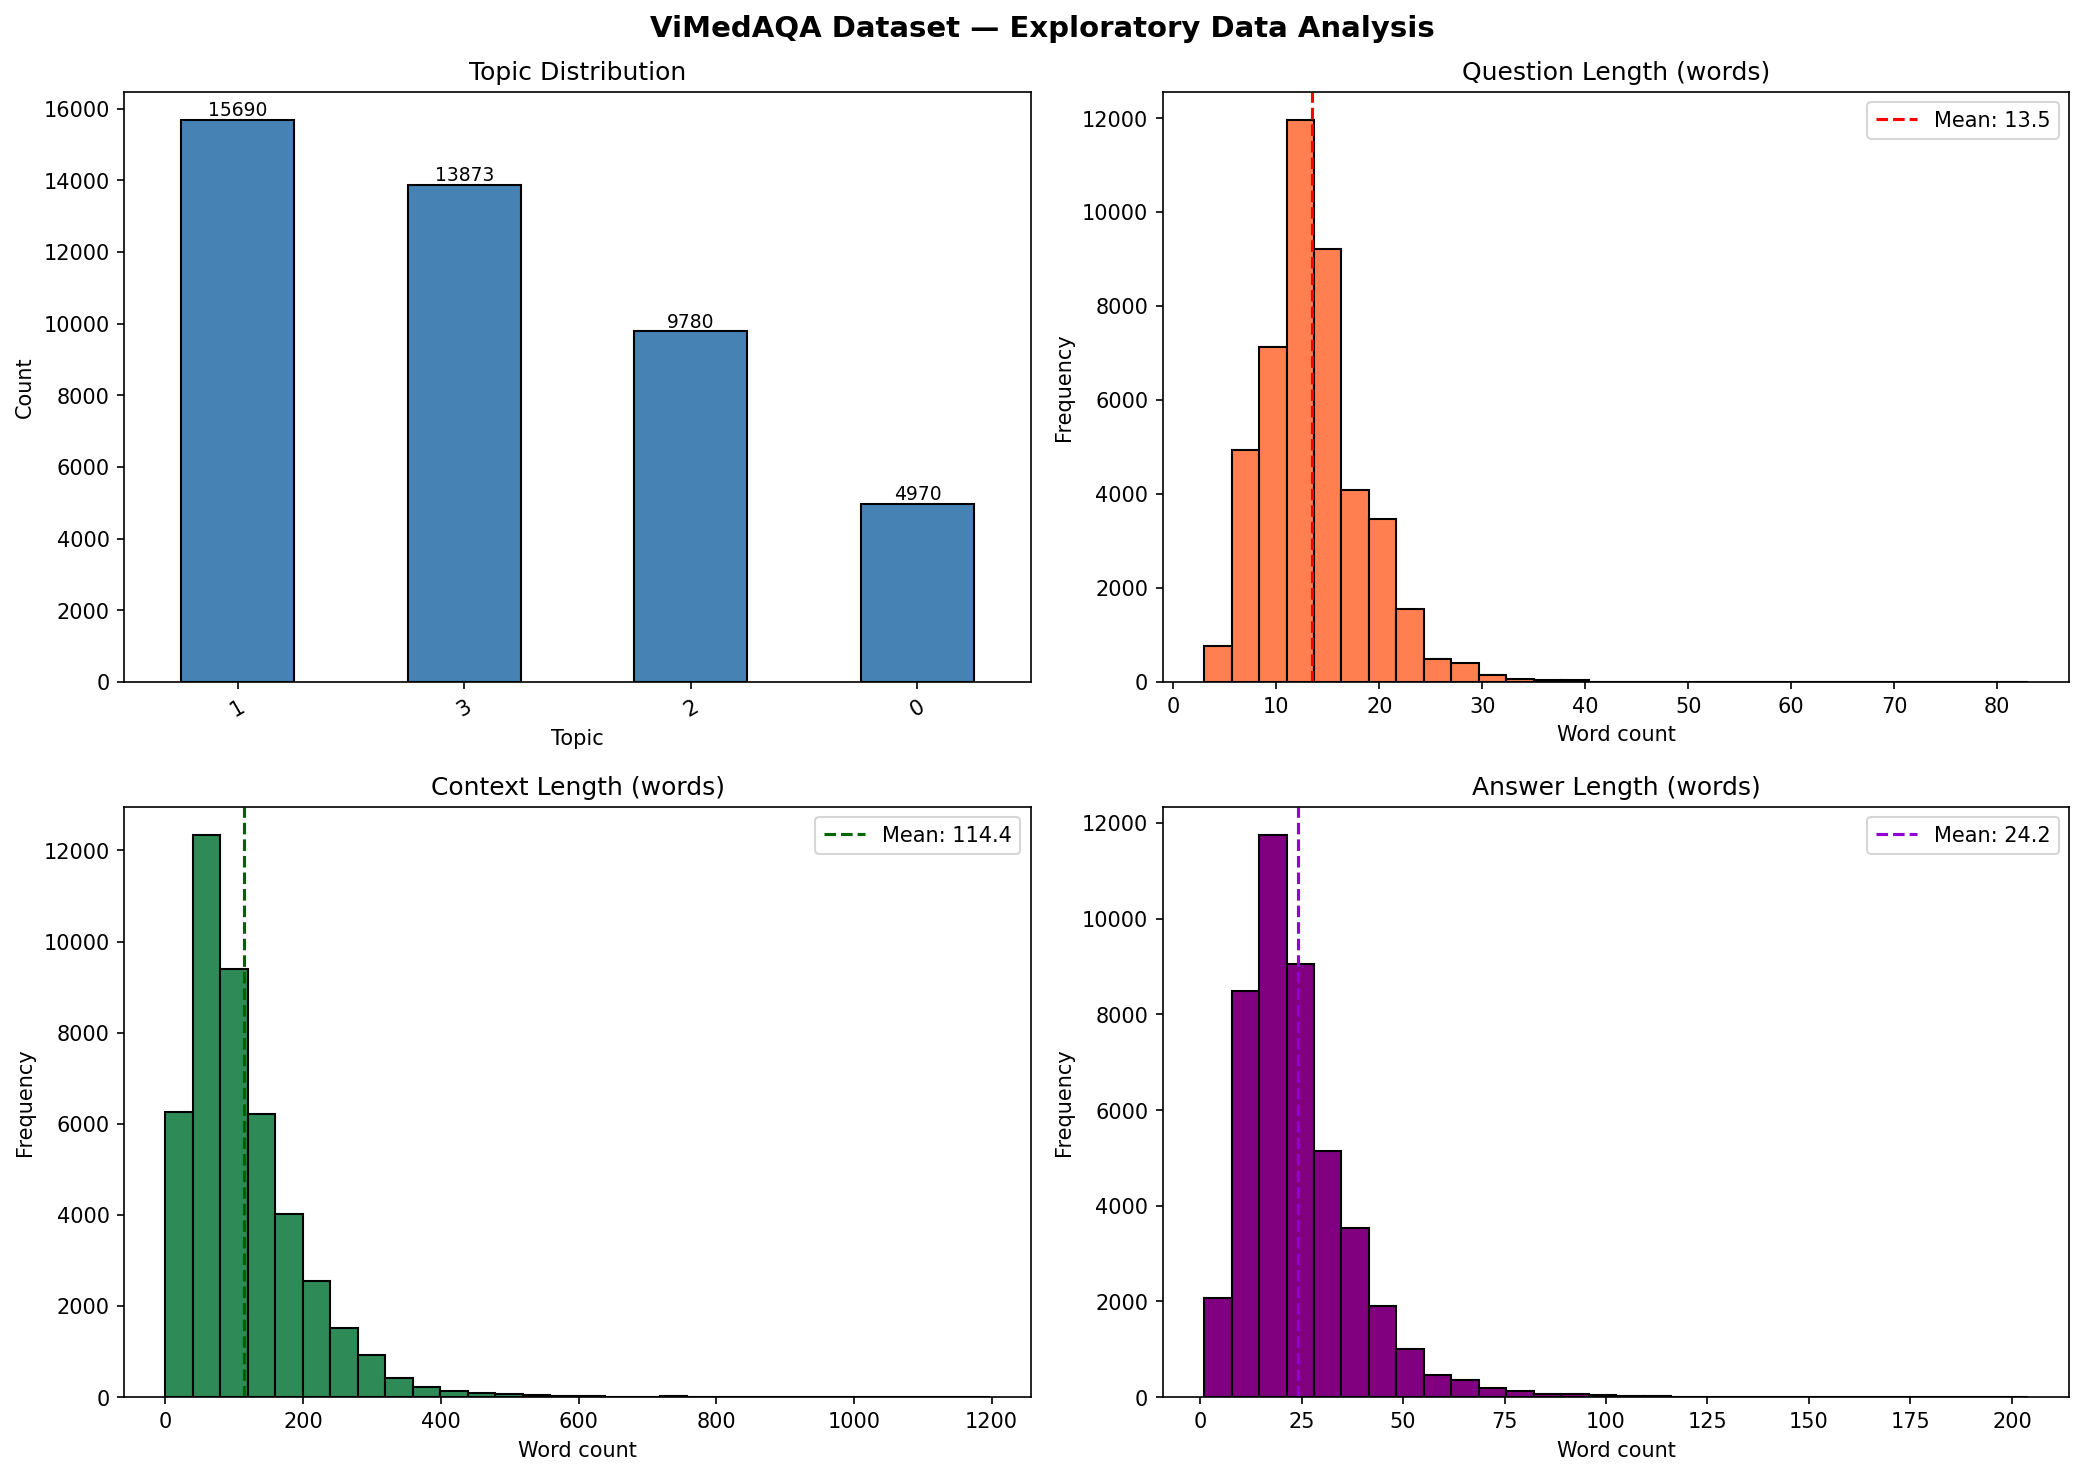
\includegraphics[width=0.85\textwidth]{figures/length_distributions.png}
    \caption{Phân phối độ dài câu hỏi, ngữ cảnh và câu trả lời trong bộ dữ liệu ViMedAQA}
    \label{fig:length_dist}
\end{figure}

Từ biểu đồ Hình~\ref{fig:length_dist}, có thể quan sát thấy phân phối độ dài câu hỏi tập trung rất ngắn (đa số dưới 50 từ), phù hợp với hành vi đặt câu hỏi tự nhiên của người bệnh. Câu trả lời cũng được tối ưu hóa độ dài trong khoảng từ 20 đến 100 từ nhằm đảm bảo tính súc tích, tránh lan man. Ngược lại, ngữ cảnh y học có phân phối trải rộng hơn và có đuôi dài (long-tail) lên đến hơn 500 từ. Phân phối này đòi hỏi các mô hình sinh chuỗi phải có khả năng biểu diễn ngữ cảnh dài hiệu quả mà không bị suy giảm khả năng tập trung (attention distraction).

\section{Chia tập dữ liệu phân tầng (Stratified Split)}
Để đảm bảo quá trình huấn luyện và đánh giá không bị sai lệch do mất cân bằng phân phối giữa các tập dữ liệu con, chúng tôi áp dụng kỹ thuật chia dữ liệu phân tầng (\textbf{Stratified Split}) dựa trên nhãn kết hợp giữa chủ đề y khoa (\texttt{topic}) và loại câu hỏi (\texttt{question\_type}) với giá trị seed cố định là \texttt{42}. Quy trình này giúp giữ nguyên tỷ lệ phân phối của từng lớp chủ đề trong cả ba tập huấn luyện, kiểm định và kiểm thử, ngăn ngừa hiện tượng dịch chuyển phân phối (distribution shift) vốn là tác nhân chính gây suy giảm độ ổn định của mô hình khi triển khai thực tế. Quy trình dọn dẹp dữ liệu cũng đã loại bỏ hoàn toàn các mẫu trùng lặp và rò rỉ dữ liệu (data leakage) giữa tập huấn luyện và tập kiểm thử, đảm bảo kết quả thực nghiệm hoàn toàn khách quan.